\documentclass[ %handout, % for handouts %%% 12pt,handout,
 10pt, xcolor={dvipsnames,svgnames,x11names,hyperref},
   hyperref={colorlinks=true,citecolor=green,linkcolor=DarkRed,urlcolor=ProcessBlue,anchorcolor=blue}
  ]{beamer}
\usepackage[ruled, linesnumbered]{algorithm2e}

\usepackage{tcolorbox}
 \tcbuselibrary{skins,raster}
\usepackage{outlines}
\usepackage{multirow}
\usepackage{babel}
\usepackage{xcolor}
\usepackage{blindtext}
\usepackage{verbatim}
\usepackage{minted}


\usepackage{pgfplots}
\pgfplotsset{compat=1.14}
\usepgfplotslibrary{statistics}

\setbeamertemplate{navigation symbols}{}

 \usepackage{relsize}

\usepackage{bookmark}

%\usepackage[hyperref]{xcolor}


\let\oldcite=\cite
\renewcommand{\cite}[1]{\textcolor[rgb]{.7,.7,.7}{\oldcite{#1}}}


\mode<presentation> {

% The Beamer class comes with a number of default slide themes
% which change the colors and layouts of slides. Below this is a list
% of all the themes, uncomment each in turn to see what they look like.

%\usetheme{default}
%\usetheme{AnnArbor}
%\usetheme{Antibes}
%\usetheme{Bergen}
%\usetheme{Berkeley}
%\usetheme{Berlin}
%\usetheme{Boadilla}
%\usetheme{CambridgeUS}
%\usetheme{Copenhagen}
%\usetheme{Darmstadt}
%\usetheme{Dresden}
%\usetheme{Frankfurt}
%\usetheme{Goettingen}
%\usetheme{Hannover}
%\usetheme{Ilmenau}
%\usetheme{JuanLesPins}
%\usetheme{Luebeck}
\usetheme{Madrid}
%\usetheme{Malmoe}
%\usetheme{Marburg}
%\usetheme{Montpellier}
%\usetheme{PaloAlto}
%\usetheme{Pittsburgh}
%\usetheme{Rochester}
%\usetheme{Singapore}
%\usetheme{Szeged}
%\usetheme{Warsaw}

% As well as themes, the Beamer class has a number of color themes
% for any slide theme. Uncomment each of these in turn to see how it
% changes the colors of your current slide theme.

%\usecolortheme{albatross}
%\usecolortheme{beaver}
%\usecolortheme{beetle}
%\usecolortheme{crane}
\usecolortheme{dolphin}
%\usecolortheme{dove}
%\usecolortheme{fly}
%\usecolortheme{lily}
%\usecolortheme{orchid}
%\usecolortheme{rose}
%\usecolortheme{seagull}
%\usecolortheme{seahorse}
%\usecolortheme{whale}
%\usecolortheme{wolverine}

%\setbeamertemplate{footline} % To remove the footer line in all slides uncomment this line
%\setbeamertemplate{footline}[page number] % To replace the footer line in all slides with a simple slide count uncomment this line

%\setbeamertemplate{navigation symbols}{} % To remove the navigation symbols from the bottom of all slides uncomment this line
}

\setbeamercolor{alerted text}{fg=red}


\usepackage[absolute,overlay]{textpos}
\usepackage{graphicx}
\usepackage{booktabs} % Allows the use of \toprule, \midrule and \bottomrule in tables
\usepackage{forest}
 \usepackage{tikz}
 \usetikzlibrary{shapes.geometric}
\usepackage{rotating}
\usepackage[]{wrapfig}
\usetikzlibrary{arrows,shapes}
\usetikzlibrary{trees,matrix}
\usepackage{multirow}
\usepackage{dirtree}
%\usepackage{color, colortbl}
\definecolor{Gray}{gray}{0.85}
\newcommand\x{.11}
\graphicspath{ {Images/} }
\usepackage{mathrsfs}
%\usepackage[symbol]{footmisc}

%\usepackage{xcolor}
%\hypersetup{
%  colorlinks,
%  allcolors=.,
%  urlcolor=ProcessBlue,
%}
%\hypersetup{colorlinks = true,
%%            linkcolor = red,
 %           urlcolor=ProcessBlue,
 %           citecolor = green,
 %           anchorcolor = blue}

%\usepackage{bibunits}
%\setbeamertemplate{bibliography item}{[\theenumiv]}
%\defaultbibliography{IoT,CPS}
%\defaultbibliographystyle{IEEEtran}

\usepackage[numbers]{natbib}
\usepackage{bibunits}

%If by "animated" you mean creating overlays, then a straight application of Daniel's visible on key would solve the problem.
%Step 1. Put the following in the preamble:
\tikzset{
    invisible/.style={opacity=0,text opacity=0},
    visible on/.style={alt=#1{}{invisible}},
    alt/.code args={<#1>#2#3}{%
      \alt<#1>{\pgfkeysalso{#2}}{\pgfkeysalso{#3}} % \pgfkeysalso doesn't change the path
    },
}
\forestset{
  visible on/.style={
    %for children={
      /tikz/visible on={#1},
      edge={/tikz/visible on={#1}}
   % }
  }
}


\AtBeginSection[]
{
  \begin{frame}<beamer>
    \frametitle{Outline}
    \tableofcontents[currentsection]
  \end{frame}
}

\AtBeginSubsection[]
{
  \begin{frame}<beamer>
    \frametitle{Outline}
    \tableofcontents[currentsubsection]
  \end{frame}
}

% \logo{\raisebox{-0.5cm}{\includegraphics[width=1cm]{naulogo.png}}\hspace*{0.5cm}}

\newenvironment{stepitemize}{\begin{itemize}[<+->]}{\end{itemize} }

\newcommand{\myblue}{\only{\color{blue}}}
\newcommand{\mygreen}{\only{\color{green}}}
\newcommand{\myyellow}{\only{\color{yellow}}}
\newcommand{\myorange}{\only{\color{orange}}}
\newcommand{\myred}{\only{\color{red}}}
\newcommand{\Z}{\mathbb{Z}}
\newcommand{\Q}{\mathbb{Q}}
\newcommand{\R}{\mathbb{R}}
\newcommand{\C}{\mathbb{C}}
\newcommand{\RR}{\mbox{\msbm R}}
\newcommand{\F}{\mathbb{F}}
\newcommand{\Rs}{\mathcal{R}}
\newcommand{\Hs}{\mathbb{H}}

\begin{document}

\title[Number Theory Fundamentals]{
Groups Fundamentals for Homomorphic Encryption}
\author{Bahattin Yildiz}
\institute[DBIO-Glade]{DBIO-Glade}
\date[September]{September 2022}
\maketitle

\section{Introduction}

\begin{frame}\frametitle{Introduction}

\begin{quote}
{ ``All of Mathematics is a tale about groups.". (Henri Poincar\'e)}
\end{quote}

\bigskip
\noindent
\begin{center}
    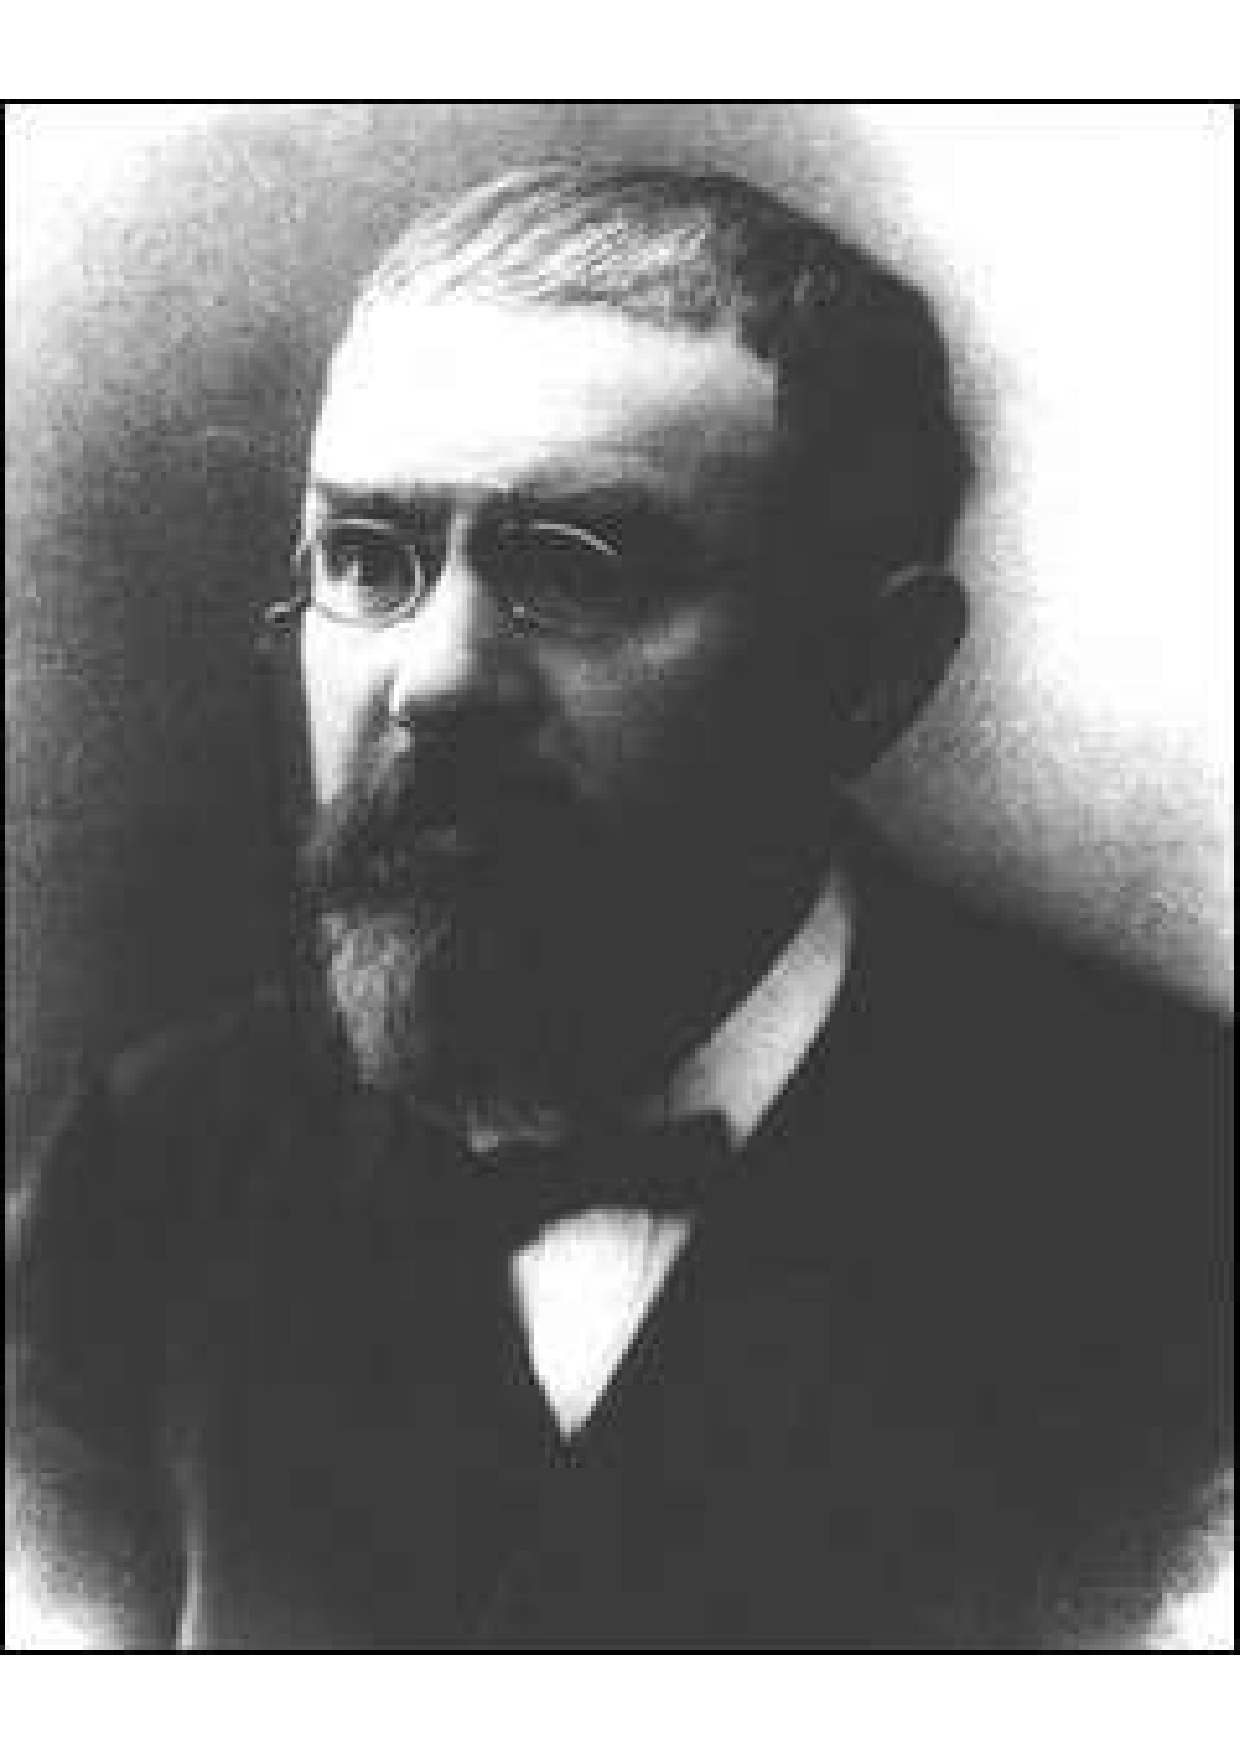
\includegraphics[scale=.20]{images/poincare_henri1.pdf}
\end{center}
\end{frame}
\begin{frame}{Why Groups?}
\begin{stepitemize}
    \item Almost every structure we see in HE has a group structure
    \item For example, $\Z$, $\Z_q$, $\Z[x]$, $\R$, $\C$, $\Z[x]/(\Phi_m(x))$, $\Z_q[x]/(f(x))$ are all groups.
    \item Moreover the set of field automorphisms which play a crucial role in slot permutations is also a group.
    \item Groups are a fundamental structure in all the subsequent topics related to rings and fields and hence are needed to understand all these topics.
    \item Before formalizing the concept of a group, we will see some motivating examples.
\end{stepitemize}
\end{frame}

\begin{frame}{A ``tale" of shifts}
\begin{stepitemize}
    \item  Consider the following action on a sequence $a_1, a_2, \dots, a_n$.
    \item We take $a_n$ from the end and bring it to the beginning, shifting everything else to the right.
    \item Let us denote this ``thing" by $\tau$.
    \item So essentially we can say $\tau([a_1, a_2, \dots, a_n]) = [a_n, a_1, a_2, \dots, a_{n-1}]$.
    \item Of course it can be applied many times.
    \item Let us denote the multiple applications by $\tau^k$. So that
    $$\tau^2([a_1, a_2, \dots, a_n]) = \tau(\tau([a_1, a_2, \dots, a_n]))=[a_{n-1},a_{n},a_1, \dots, a_{n-2}].$$
\end{stepitemize}
\end{frame}

\begin{frame}{$\tau$ and its powers in action}
\begin{stepitemize}
    \item Here is an example on $5$ elements. We will represent $a_i$ by different colors.
    \item[]

\bigskip

\begin{center}
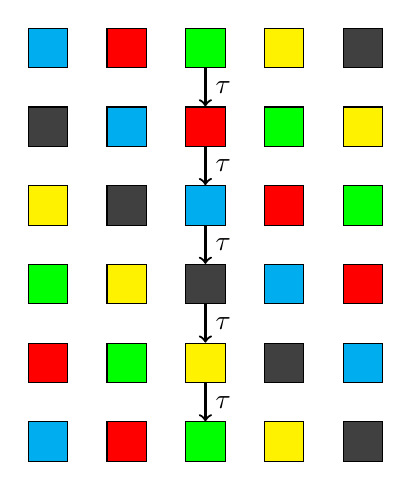
\begin{tikzpicture}

 \node[fill=cyan, text=black, rectangle,draw,  minimum width = 0.5cm,
    minimum height = 0.5cm] (r1) at (0,0) {};

 \node[fill=red, text=black, rectangle,draw,  minimum width = 0.5cm,
    minimum height = 0.5cm] (r2) at (1,0) {};

 \node[fill=green, text=black, rectangle,draw,  minimum width = 0.5cm,
    minimum height = 0.5cm] (r3) at (2,0) {};

\node[fill=yellow, text=black, rectangle,draw,  minimum width = 0.5cm,
    minimum height = 0.5cm] (r4) at (3,0) {};

\node[fill=darkgray, text=black, rectangle,draw,  minimum width = 0.5cm,
    minimum height = 0.5cm] (r5) at (4,0) {};

 \node[fill=darkgray, text=black, rectangle,draw,  minimum width = 0.5cm,
    minimum height = 0.5cm] (q1) at (0,-1) {};

 \node[fill=cyan, text=black, rectangle,draw,  minimum width = 0.5cm,
    minimum height = 0.5cm] (q2) at (1,-1) {};

 \node[fill=red, text=black, rectangle,draw,  minimum width = 0.5cm,
    minimum height = 0.5cm] (q3) at (2,-1) {};

\node[fill=green, text=black, rectangle,draw,  minimum width = 0.5cm,
    minimum height = 0.5cm] (q4) at (3,-1) {};

\node[fill=yellow, text=black, rectangle,draw,  minimum width = 0.5cm,
    minimum height = 0.5cm] (q5) at (4,-1) {};
\draw [thick, ->] (r3) -- (q3) node[midway, right] {$\tau$};

 \node[fill=yellow, text=black, rectangle,draw,  minimum width = 0.5cm,
    minimum height = 0.5cm] (s1) at (0,-2) {};

 \node[fill=darkgray, text=black, rectangle,draw,  minimum width = 0.5cm,
    minimum height = 0.5cm] (s2) at (1,-2) {};

 \node[fill=cyan, text=black, rectangle,draw,  minimum width = 0.5cm,
    minimum height = 0.5cm] (s3) at (2,-2) {};

\node[fill=red, text=black, rectangle,draw,  minimum width = 0.5cm,
    minimum height = 0.5cm] (s4) at (3,-2) {};

\node[fill=green, text=black, rectangle,draw,  minimum width = 0.5cm,
    minimum height = 0.5cm] (s5) at (4,-2) {};
\draw [thick, ->] (q3) -- (s3) node[midway, right] {$\tau$};

 \node[fill=green, text=black, rectangle,draw,  minimum width = 0.5cm,
    minimum height = 0.5cm] (t1) at (0,-3) {};

 \node[fill=yellow, text=black, rectangle,draw,  minimum width = 0.5cm,
    minimum height = 0.5cm] (t2) at (1,-3) {};

 \node[fill=darkgray, text=black, rectangle,draw,  minimum width = 0.5cm,
    minimum height = 0.5cm] (t3) at (2,-3) {};

\node[fill=cyan, text=black, rectangle,draw,  minimum width = 0.5cm,
    minimum height = 0.5cm] (t4) at (3,-3) {};

\node[fill=red, text=black, rectangle,draw,  minimum width = 0.5cm,
    minimum height = 0.5cm] (t5) at (4,-3) {};
\draw [thick, ->] (s3) -- (t3) node[midway, right] {$\tau$};


 \node[fill=red, text=black, rectangle,draw,  minimum width = 0.5cm,
    minimum height = 0.5cm] (u1) at (0,-4) {};

 \node[fill=green, text=black, rectangle,draw,  minimum width = 0.5cm,
    minimum height = 0.5cm] (u2) at (1,-4) {};

 \node[fill=yellow, text=black, rectangle,draw,  minimum width = 0.5cm,
    minimum height = 0.5cm] (u3) at (2,-4) {};

\node[fill=darkgray, text=black, rectangle,draw,  minimum width = 0.5cm,
    minimum height = 0.5cm] (u4) at (3,-4) {};

\node[fill=cyan, text=black, rectangle,draw,  minimum width = 0.5cm,
    minimum height = 0.5cm] (u5) at (4,-4) {};
\draw [thick, ->] (t3) -- (u3) node[midway, right] {$\tau$};


 \node[fill=cyan, text=black, rectangle,draw,  minimum width = 0.5cm,
    minimum height = 0.5cm] (v1) at (0,-5) {};

 \node[fill=red, text=black, rectangle,draw,  minimum width = 0.5cm,
    minimum height = 0.5cm] (v2) at (1,-5) {};

 \node[fill=green, text=black, rectangle,draw,  minimum width = 0.5cm,
    minimum height = 0.5cm] (v3) at (2,-5) {};

\node[fill=yellow, text=black, rectangle,draw,  minimum width = 0.5cm,
    minimum height = 0.5cm] (v4) at (3,-5) {};

\node[fill=darkgray, text=black, rectangle,draw,  minimum width = 0.5cm,
    minimum height = 0.5cm] (v5) at (4,-5) {};
\draw [thick, ->] (u3) -- (v3) node[midway, right] {$\tau$};

\end{tikzpicture}
\end{center}
\end{stepitemize}
\end{frame}

\begin{frame}
\begin{stepitemize}
    \item So, what happened? We see that when we applied $\tau$ $5$ times, we got the original configuration.
    \item That is
    $$\tau^5([\textrm{cyan, red, grn, yellow, gray}]) = [\textrm{cyan, red, grn, yellow, gray}].$$
    \item So $\tau^5$ is an ``action" that does not change anything, or as we will call it later, leaves the configuration ``fixed".
\end{stepitemize}
\end{frame}

\begin{frame}{A second ``shift"}
\begin{stepitemize}
\item Now let us consider a different ``action" on $[a_1, a_2, \dots, a_n]$
\item We denote it by $\sigma$
\item $\sigma$ is also a shift but it is a ``left shift".
\item That is $\sigma$ takes the leftmost term and appends it to the end, while shifting every other element one unit towards the left.
\item So
$$\sigma([a_1, a_2, \dots, a_n]) = [a_2, a_3, \dots, a_n, a_1]. $$
\item So let us see $\sigma$ in action on the same configuration that we saw above.
\end{stepitemize}
\end{frame}

\begin{frame}{$\sigma$ and its powers in action}

\begin{center}
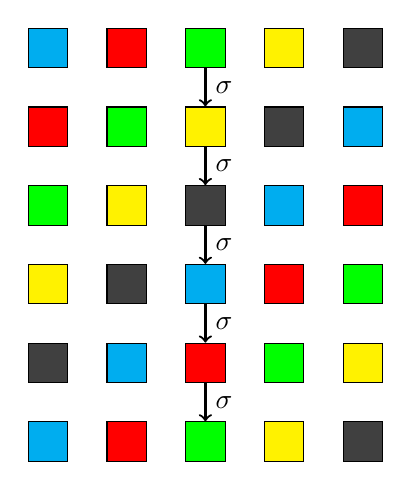
\begin{tikzpicture}

 \node[fill=cyan, text=black, rectangle,draw,  minimum width = 0.5cm,
    minimum height = 0.5cm] (r1) at (0,0) {};

 \node[fill=red, text=black, rectangle,draw,  minimum width = 0.5cm,
    minimum height = 0.5cm] (r2) at (1,0) {};

 \node[fill=green, text=black, rectangle,draw,  minimum width = 0.5cm,
    minimum height = 0.5cm] (r3) at (2,0) {};

\node[fill=yellow, text=black, rectangle,draw,  minimum width = 0.5cm,
    minimum height = 0.5cm] (r4) at (3,0) {};

\node[fill=darkgray, text=black, rectangle,draw,  minimum width = 0.5cm,
    minimum height = 0.5cm] (r5) at (4,0) {};

 \node[fill=red, text=black, rectangle,draw,  minimum width = 0.5cm,
    minimum height = 0.5cm] (q1) at (0,-1) {};

 \node[fill=green, text=black, rectangle,draw,  minimum width = 0.5cm,
    minimum height = 0.5cm] (q2) at (1,-1) {};

 \node[fill=yellow, text=black, rectangle,draw,  minimum width = 0.5cm,
    minimum height = 0.5cm] (q3) at (2,-1) {};

\node[fill=darkgray, text=black, rectangle,draw,  minimum width = 0.5cm,
    minimum height = 0.5cm] (q4) at (3,-1) {};

\node[fill=cyan, text=black, rectangle,draw,  minimum width = 0.5cm,
    minimum height = 0.5cm] (q5) at (4,-1) {};
\draw [thick, ->] (r3) -- (q3) node[midway, right] {$\sigma$};

 \node[fill=green, text=black, rectangle,draw,  minimum width = 0.5cm,
    minimum height = 0.5cm] (s1) at (0,-2) {};

 \node[fill=yellow, text=black, rectangle,draw,  minimum width = 0.5cm,
    minimum height = 0.5cm] (s2) at (1,-2) {};

 \node[fill=darkgray, text=black, rectangle,draw,  minimum width = 0.5cm,
    minimum height = 0.5cm] (s3) at (2,-2) {};

\node[fill=cyan, text=black, rectangle,draw,  minimum width = 0.5cm,
    minimum height = 0.5cm] (s4) at (3,-2) {};

\node[fill=red, text=black, rectangle,draw,  minimum width = 0.5cm,
    minimum height = 0.5cm] (s5) at (4,-2) {};
\draw [thick, ->] (q3) -- (s3) node[midway, right] {$\sigma$};

 \node[fill=yellow, text=black, rectangle,draw,  minimum width = 0.5cm,
    minimum height = 0.5cm] (t1) at (0,-3) {};

 \node[fill=darkgray, text=black, rectangle,draw,  minimum width = 0.5cm,
    minimum height = 0.5cm] (t2) at (1,-3) {};

 \node[fill=cyan, text=black, rectangle,draw,  minimum width = 0.5cm,
    minimum height = 0.5cm] (t3) at (2,-3) {};

\node[fill=red, text=black, rectangle,draw,  minimum width = 0.5cm,
    minimum height = 0.5cm] (t4) at (3,-3) {};

\node[fill=green, text=black, rectangle,draw,  minimum width = 0.5cm,
    minimum height = 0.5cm] (t5) at (4,-3) {};
\draw [thick, ->] (s3) -- (t3) node[midway, right] {$\sigma$};


 \node[fill=darkgray, text=black, rectangle,draw,  minimum width = 0.5cm,
    minimum height = 0.5cm] (u1) at (0,-4) {};

 \node[fill=cyan, text=black, rectangle,draw,  minimum width = 0.5cm,
    minimum height = 0.5cm] (u2) at (1,-4) {};

 \node[fill=red, text=black, rectangle,draw,  minimum width = 0.5cm,
    minimum height = 0.5cm] (u3) at (2,-4) {};

\node[fill=green, text=black, rectangle,draw,  minimum width = 0.5cm,
    minimum height = 0.5cm] (u4) at (3,-4) {};

\node[fill=yellow, text=black, rectangle,draw,  minimum width = 0.5cm,
    minimum height = 0.5cm] (u5) at (4,-4) {};
\draw [thick, ->] (t3) -- (u3) node[midway, right] {$\sigma$};


 \node[fill=cyan, text=black, rectangle,draw,  minimum width = 0.5cm,
    minimum height = 0.5cm] (v1) at (0,-5) {};

 \node[fill=red, text=black, rectangle,draw,  minimum width = 0.5cm,
    minimum height = 0.5cm] (v2) at (1,-5) {};

 \node[fill=green, text=black, rectangle,draw,  minimum width = 0.5cm,
    minimum height = 0.5cm] (v3) at (2,-5) {};

\node[fill=yellow, text=black, rectangle,draw,  minimum width = 0.5cm,
    minimum height = 0.5cm] (v4) at (3,-5) {};

\node[fill=darkgray, text=black, rectangle,draw,  minimum width = 0.5cm,
    minimum height = 0.5cm] (v5) at (4,-5) {};
\draw [thick, ->] (u3) -- (v3) node[midway, right] {$\sigma$};

\end{tikzpicture}
\end{center}
\end{frame}
\begin{frame}
\begin{stepitemize}
    \item We see a similar behaviour in $\sigma$ as well.
    \item Just like $\tau$, we came back to the original configuration after applying $\sigma $ $5$ times.
    \item Namely,
$$\sigma^5([\textrm{cyan, red, grn, yellow, gray}]) = [\textrm{cyan, red, grn, yellow, gray}].$$
    \item But is that the only common ground between $\tau$ and $\sigma$?
    \item To see what happens let us look at what happens when we apply $\sigma$ and $\tau$ successively.
\end{stepitemize}

\end{frame}

\begin{frame}{$\sigma$ vs $\tau$}

\begin{stepitemize}
\item[]
\begin{center}
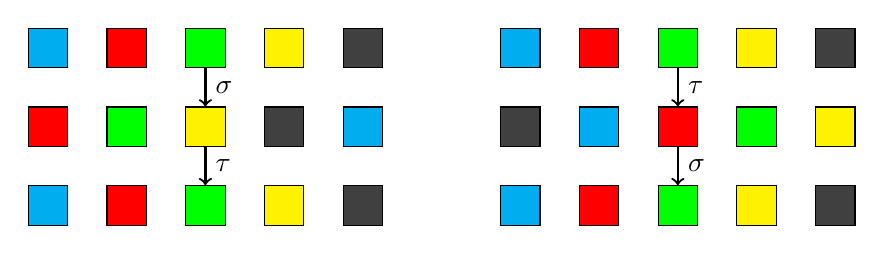
\begin{tikzpicture}

 \node[fill=cyan, text=black, rectangle,draw,  minimum width = 0.5cm,
    minimum height = 0.5cm] (r1) at (0,0) {};

 \node[fill=red, text=black, rectangle,draw,  minimum width = 0.5cm,
    minimum height = 0.5cm] (r2) at (1,0) {};

 \node[fill=green, text=black, rectangle,draw,  minimum width = 0.5cm,
    minimum height = 0.5cm] (r3) at (2,0) {};

\node[fill=yellow, text=black, rectangle,draw,  minimum width = 0.5cm,
    minimum height = 0.5cm] (r4) at (3,0) {};

\node[fill=darkgray, text=black, rectangle,draw,  minimum width = 0.5cm,
    minimum height = 0.5cm] (r5) at (4,0) {};

 \node[fill=red, text=black, rectangle,draw,  minimum width = 0.5cm,
    minimum height = 0.5cm] (q1) at (0,-1) {};

 \node[fill=green, text=black, rectangle,draw,  minimum width = 0.5cm,
    minimum height = 0.5cm] (q2) at (1,-1) {};

 \node[fill=yellow, text=black, rectangle,draw,  minimum width = 0.5cm,
    minimum height = 0.5cm] (q3) at (2,-1) {};

\node[fill=darkgray, text=black, rectangle,draw,  minimum width = 0.5cm,
    minimum height = 0.5cm] (q4) at (3,-1) {};

\node[fill=cyan, text=black, rectangle,draw,  minimum width = 0.5cm,
    minimum height = 0.5cm] (q5) at (4,-1) {};
\draw [thick, ->] (r3) -- (q3) node[midway, right] {$\sigma$};

\node[fill=cyan, text=black, rectangle,draw,  minimum width = 0.5cm,
    minimum height = 0.5cm] (s1) at (0,-2) {};

 \node[fill=red, text=black, rectangle,draw,  minimum width = 0.5cm,
    minimum height = 0.5cm] (s2) at (1,-2) {};

 \node[fill=green, text=black, rectangle,draw,  minimum width = 0.5cm,
    minimum height = 0.5cm] (s3) at (2,-2) {};

\node[fill=yellow, text=black, rectangle,draw,  minimum width = 0.5cm,
    minimum height = 0.5cm] (s4) at (3,-2) {};

\node[fill=darkgray, text=black, rectangle,draw,  minimum width = 0.5cm,
    minimum height = 0.5cm] (s5) at (4,-2) {};

\draw [thick, ->] (q3) -- (s3) node[midway, right] {$\tau$};



 \node[fill=cyan, text=black, rectangle,draw,  minimum width = 0.5cm,
    minimum height = 0.5cm] (t1) at (6,0) {};

 \node[fill=red, text=black, rectangle,draw,  minimum width = 0.5cm,
    minimum height = 0.5cm] (t2) at (7,0) {};

 \node[fill=green, text=black, rectangle,draw,  minimum width = 0.5cm,
    minimum height = 0.5cm] (t3) at (8,0) {};

\node[fill=yellow, text=black, rectangle,draw,  minimum width = 0.5cm,
    minimum height = 0.5cm] (t4) at (9,0) {};

\node[fill=darkgray, text=black, rectangle,draw,  minimum width = 0.5cm,
    minimum height = 0.5cm] (t5) at (10,0) {};

 \node[fill=darkgray, text=black, rectangle,draw,  minimum width = 0.5cm,
    minimum height = 0.5cm] (u1) at (6,-1) {};

 \node[fill=cyan, text=black, rectangle,draw,  minimum width = 0.5cm,
    minimum height = 0.5cm] (u2) at (7,-1) {};

 \node[fill=red, text=black, rectangle,draw,  minimum width = 0.5cm,
    minimum height = 0.5cm] (u3) at (8,-1) {};

\node[fill=green, text=black, rectangle,draw,  minimum width = 0.5cm,
    minimum height = 0.5cm] (u4) at (9,-1) {};

\node[fill=yellow, text=black, rectangle,draw,  minimum width = 0.5cm,
    minimum height = 0.5cm] (u5) at (10,-1) {};
\draw [thick, ->] (t3) -- (u3) node[midway, right] {$\tau$};

\node[fill=cyan, text=black, rectangle,draw,  minimum width = 0.5cm,
    minimum height = 0.5cm] (v1) at (6,-2) {};

 \node[fill=red, text=black, rectangle,draw,  minimum width = 0.5cm,
    minimum height = 0.5cm] (v2) at (7,-2) {};

 \node[fill=green, text=black, rectangle,draw,  minimum width = 0.5cm,
    minimum height = 0.5cm] (v3) at (8,-2) {};

\node[fill=yellow, text=black, rectangle,draw,  minimum width = 0.5cm,
    minimum height = 0.5cm] (v4) at (9,-2) {};

\node[fill=darkgray, text=black, rectangle,draw,  minimum width = 0.5cm,
    minimum height = 0.5cm] (v5) at (10,-2) {};

\draw [thick, ->] (u3) -- (v3) node[midway, right] {$\sigma$};

\end{tikzpicture}
\end{center}

\bigskip

\item So what do we see?
\item $\sigma\tau = \tau\sigma$ act in exactly the same way and they both leave the configuration ``fixed".
\item This is kind of expected as the ``actions" of $\sigma$ and $\tau$ are ``opposite" of each other.
\item But that is not all. In order to see more connections, let us write the actions side by side
\end{stepitemize}
\end{frame}

\begin{frame}{More on $\sigma$ vs $\tau$}
\begin{stepitemize}
\item[]\bigskip

\begin{center}
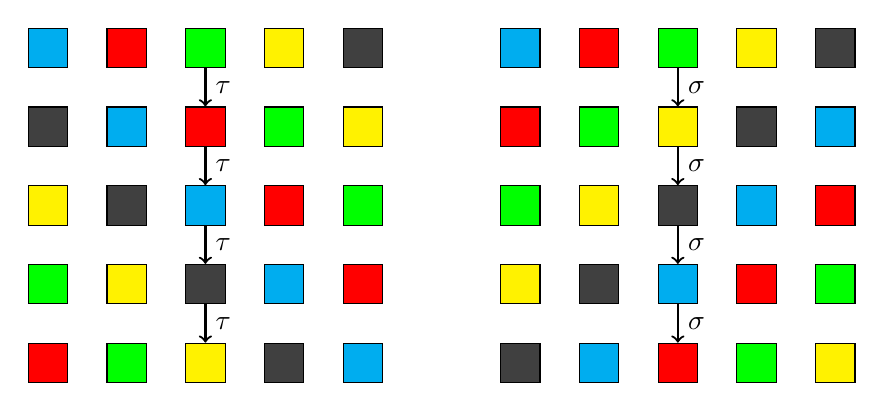
\begin{tikzpicture}

 \node[fill=cyan, text=black, rectangle,draw,  minimum width = 0.5cm,
    minimum height = 0.5cm] (r1) at (0,0) {};

 \node[fill=red, text=black, rectangle,draw,  minimum width = 0.5cm,
    minimum height = 0.5cm] (r2) at (1,0) {};

 \node[fill=green, text=black, rectangle,draw,  minimum width = 0.5cm,
    minimum height = 0.5cm] (r3) at (2,0) {};

\node[fill=yellow, text=black, rectangle,draw,  minimum width = 0.5cm,
    minimum height = 0.5cm] (r4) at (3,0) {};

\node[fill=darkgray, text=black, rectangle,draw,  minimum width = 0.5cm,
    minimum height = 0.5cm] (r5) at (4,0) {};

 \node[fill=darkgray, text=black, rectangle,draw,  minimum width = 0.5cm,
    minimum height = 0.5cm] (q1) at (0,-1) {};

 \node[fill=cyan, text=black, rectangle,draw,  minimum width = 0.5cm,
    minimum height = 0.5cm] (q2) at (1,-1) {};

 \node[fill=red, text=black, rectangle,draw,  minimum width = 0.5cm,
    minimum height = 0.5cm] (q3) at (2,-1) {};

\node[fill=green, text=black, rectangle,draw,  minimum width = 0.5cm,
    minimum height = 0.5cm] (q4) at (3,-1) {};

\node[fill=yellow, text=black, rectangle,draw,  minimum width = 0.5cm,
    minimum height = 0.5cm] (q5) at (4,-1) {};
\draw [thick, ->] (r3) -- (q3) node[midway, right] {$\tau$};

 \node[fill=yellow, text=black, rectangle,draw,  minimum width = 0.5cm,
    minimum height = 0.5cm] (s1) at (0,-2) {};

 \node[fill=darkgray, text=black, rectangle,draw,  minimum width = 0.5cm,
    minimum height = 0.5cm] (s2) at (1,-2) {};

 \node[fill=cyan, text=black, rectangle,draw,  minimum width = 0.5cm,
    minimum height = 0.5cm] (s3) at (2,-2) {};

\node[fill=red, text=black, rectangle,draw,  minimum width = 0.5cm,
    minimum height = 0.5cm] (s4) at (3,-2) {};

\node[fill=green, text=black, rectangle,draw,  minimum width = 0.5cm,
    minimum height = 0.5cm] (s5) at (4,-2) {};
\draw [thick, ->] (q3) -- (s3) node[midway, right] {$\tau$};

 \node[fill=green, text=black, rectangle,draw,  minimum width = 0.5cm,
    minimum height = 0.5cm] (t1) at (0,-3) {};

 \node[fill=yellow, text=black, rectangle,draw,  minimum width = 0.5cm,
    minimum height = 0.5cm] (t2) at (1,-3) {};

 \node[fill=darkgray, text=black, rectangle,draw,  minimum width = 0.5cm,
    minimum height = 0.5cm] (t3) at (2,-3) {};

\node[fill=cyan, text=black, rectangle,draw,  minimum width = 0.5cm,
    minimum height = 0.5cm] (t4) at (3,-3) {};

\node[fill=red, text=black, rectangle,draw,  minimum width = 0.5cm,
    minimum height = 0.5cm] (t5) at (4,-3) {};
\draw [thick, ->] (s3) -- (t3) node[midway, right] {$\tau$};


 \node[fill=red, text=black, rectangle,draw,  minimum width = 0.5cm,
    minimum height = 0.5cm] (u1) at (0,-4) {};

 \node[fill=green, text=black, rectangle,draw,  minimum width = 0.5cm,
    minimum height = 0.5cm] (u2) at (1,-4) {};

 \node[fill=yellow, text=black, rectangle,draw,  minimum width = 0.5cm,
    minimum height = 0.5cm] (u3) at (2,-4) {};

\node[fill=darkgray, text=black, rectangle,draw,  minimum width = 0.5cm,
    minimum height = 0.5cm] (u4) at (3,-4) {};

\node[fill=cyan, text=black, rectangle,draw,  minimum width = 0.5cm,
    minimum height = 0.5cm] (u5) at (4,-4) {};
\draw [thick, ->] (t3) -- (u3) node[midway, right] {$\tau$};

\node[fill=cyan, text=black, rectangle,draw,  minimum width = 0.5cm,
    minimum height = 0.5cm] (r11) at (6,0) {};

 \node[fill=red, text=black, rectangle,draw,  minimum width = 0.5cm,
    minimum height = 0.5cm] (r12) at (7,0) {};

 \node[fill=green, text=black, rectangle,draw,  minimum width = 0.5cm,
    minimum height = 0.5cm] (r13) at (8,0) {};

\node[fill=yellow, text=black, rectangle,draw,  minimum width = 0.5cm,
    minimum height = 0.5cm] (r14) at (9,0) {};

\node[fill=darkgray, text=black, rectangle,draw,  minimum width = 0.5cm,
    minimum height = 0.5cm] (r15) at (10,0) {};

 \node[fill=red, text=black, rectangle,draw,  minimum width = 0.5cm,
    minimum height = 0.5cm] (q11) at (6,-1) {};

 \node[fill=green, text=black, rectangle,draw,  minimum width = 0.5cm,
    minimum height = 0.5cm] (q12) at (7,-1) {};

 \node[fill=yellow, text=black, rectangle,draw,  minimum width = 0.5cm,
    minimum height = 0.5cm] (q13) at (8,-1) {};

\node[fill=darkgray, text=black, rectangle,draw,  minimum width = 0.5cm,
    minimum height = 0.5cm] (q14) at (9,-1) {};

\node[fill=cyan, text=black, rectangle,draw,  minimum width = 0.5cm,
    minimum height = 0.5cm] (q15) at (10,-1) {};
\draw [thick, ->] (r13) -- (q13) node[midway, right] {$\sigma$};

 \node[fill=green, text=black, rectangle,draw,  minimum width = 0.5cm,
    minimum height = 0.5cm] (s11) at (6,-2) {};

 \node[fill=yellow, text=black, rectangle,draw,  minimum width = 0.5cm,
    minimum height = 0.5cm] (s12) at (7,-2) {};

 \node[fill=darkgray, text=black, rectangle,draw,  minimum width = 0.5cm,
    minimum height = 0.5cm] (s13) at (8,-2) {};

\node[fill=cyan, text=black, rectangle,draw,  minimum width = 0.5cm,
    minimum height = 0.5cm] (s14) at (9,-2) {};

\node[fill=red, text=black, rectangle,draw,  minimum width = 0.5cm,
    minimum height = 0.5cm] (s15) at (10,-2) {};
\draw [thick, ->] (q13) -- (s13) node[midway, right] {$\sigma$};

 \node[fill=yellow, text=black, rectangle,draw,  minimum width = 0.5cm,
    minimum height = 0.5cm] (t11) at (6,-3) {};

 \node[fill=darkgray, text=black, rectangle,draw,  minimum width = 0.5cm,
    minimum height = 0.5cm] (t12) at (7,-3) {};

 \node[fill=cyan, text=black, rectangle,draw,  minimum width = 0.5cm,
    minimum height = 0.5cm] (t13) at (8,-3) {};

\node[fill=red, text=black, rectangle,draw,  minimum width = 0.5cm,
    minimum height = 0.5cm] (t14) at (9,-3) {};

\node[fill=green, text=black, rectangle,draw,  minimum width = 0.5cm,
    minimum height = 0.5cm] (t5) at (10,-3) {};
\draw [thick, ->] (s13) -- (t13) node[midway, right] {$\sigma$};


 \node[fill=darkgray, text=black, rectangle,draw,  minimum width = 0.5cm,
    minimum height = 0.5cm] (u11) at (6,-4) {};

 \node[fill=cyan, text=black, rectangle,draw,  minimum width = 0.5cm,
    minimum height = 0.5cm] (u12) at (7,-4) {};

 \node[fill=red, text=black, rectangle,draw,  minimum width = 0.5cm,
    minimum height = 0.5cm] (u13) at (8,-4) {};

\node[fill=green, text=black, rectangle,draw,  minimum width = 0.5cm,
    minimum height = 0.5cm] (u14) at (9,-4) {};

\node[fill=yellow, text=black, rectangle,draw,  minimum width = 0.5cm,
    minimum height = 0.5cm] (u15) at (10,-4) {};
\draw [thick, ->] (t13) -- (u13) node[midway, right] {$\sigma$};


\end{tikzpicture}
\end{center}
\item So what do we observe?
\item Applying $\tau$ once is the same action as applying $\sigma$ four times, that is $\tau=\sigma^4$.
\item Similarly we have $\tau^2=\sigma^3$,  $\tau^3=\sigma^2$ and $\tau^4=\sigma$.
\end{stepitemize}
\end{frame}

\begin{frame}{Last words on $\sigma$ and $\tau$}

\begin{stepitemize}
\item Notice that applying $\sigma^6$ and $\sigma$ gives us the same result since $\sigma^5$ brings us back to the original.
\item The same is true for $\tau$.
\item Similarly $\tau^7=\tau^2$, $\tau^8=\tau^3$ and so on.
\item So both $\{\tau, \tau^2, \tau^3, \tau^4, \tau^5\}$ and
$\{\sigma, \sigma^2, \sigma^3, \sigma^4, \sigma^5\}$ are ``complete sets".
\item $\sigma$ being the ``opposite" of $\tau$ will be denoted by $\sigma=\tau^{-1}$, which was also $\tau^4$.
\item So we can say $\{\tau^n|n\in \Z\} = \{\tau, \tau^2, \tau^3, \tau^4, \tau^5\}$.
\item So, what we have seen is the foundation of a very simple group, that is the cyclic group of order $5$.
\end{stepitemize}
\end{frame}
\begin{frame}{Operation Table}
\begin{stepitemize}
\item Letting $G = \{1, \tau, \tau^2, \tau^3, \tau^4\}$, with the understanding that $\tau^5=1$, which is the ``identity action" that doesn't change the configuration, we can write the operation table, that visualizes the ``completenetss" of the set.

\bigskip

\item[]
\begin{table}[H]
\begin{tabular}{ c| c | c |c|c|c}
$.$  & $1$ & $\tau$ & $\tau^2$ & $\tau^3$ & $\tau^4$ \\
\hline
$1$ & $1$ & $\tau$ & $\tau^2$ & $\tau^3$ & $\tau^4$ \\
\hline
$\tau$ & $\tau$ & $\tau^2$ & $\tau^3$ & $\tau^4$ & $1$ \\
\hline
$\tau^2$ & $\tau^2$ & $\tau^3$ & $\tau^4$ & $1$ & $\tau$ \\
\hline
$\tau^3$ & $\tau^3$& $\tau^4$ & $1$&$\tau$& $\tau^2$\\
\hline
$\tau^4$ & $\tau^4$& $1$ & $\tau$&$\tau^2$& $\tau^3$\\
\end{tabular}
\end{table}
\end{stepitemize}

\end{frame}
\begin{frame}{A ``tale" of symmetries}
    \begin{stepitemize}
    \item We can consider a slightly more complex example.
\item Let us consider a ``labeled pentagon" and the symmetries that leave this pentagon intact.
\item We will consider two main operations: Rotation ($R$) and Mirror Reflection ($M$) with respect to one of the axis of symmetry.
\item To be precise, let us agree that we will rotate clock-wise by $72$ degrees and the mirror imaging will be done based on an axis of symmetry that passes through the point $A$.
\item Let us visually describe how these two operations work:
    \end{stepitemize}
\end{frame}

\begin{frame}{Visual of $R$ and $M$}
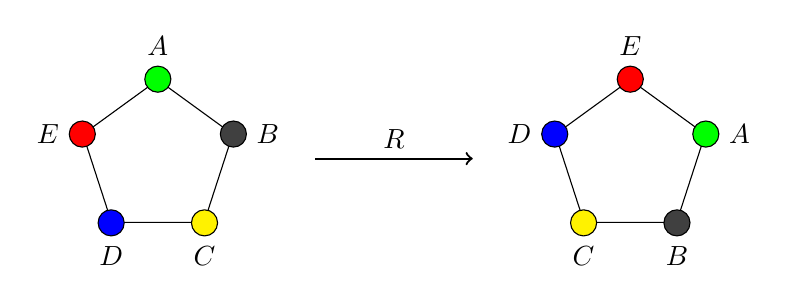
\begin{tikzpicture}
\node[minimum size=2cm,draw,regular polygon,regular polygon sides=5] at (0,0) (a) {};
\node[circle,fill=green,radius=.1cm,draw,
    label=above:{$A$}] at (a.corner 1) {};
\node[circle,fill=red, radius=.1cm,draw,
    label=left:{$E$}] at (a.corner 2) {};
\node[circle, fill=blue, radius=.1cm,draw,
    label=below:{$D$}] at (a.corner 3) {};
\node[circle,fill=yellow,radius=.1cm,draw,
    label=below:{$C$}] at (a.corner 4) {};
\node[circle,fill=darkgray,radius=.1cm,draw,
    label=right:{$B$}] at (a.corner 5) {};


\node[minimum size=2cm,draw,regular polygon,regular polygon sides=5] at (6,0) (b) {};
\node[circle,fill=red,radius=.1cm,draw,
    label=above:{$E$}] at (b.corner 1) {};
\node[circle,fill=blue, radius=.1cm,draw,
    label=left:{$D$}] at (b.corner 2) {};
\node[circle, fill=yellow, radius=.1cm,draw,
    label=below:{$C$}] at (b.corner 3) {};
\node[circle,fill=darkgray,radius=.1cm,draw,
    label=below:{$B$}] at (b.corner 4) {};
\node[circle,fill=green,radius=.1cm,draw,
    label=right:{$A$}] at (b.corner 5) {};

\draw [thick, ->] (2,0) -- (4,0) node[midway, above] {$R$};
\end{tikzpicture}


\bigskip

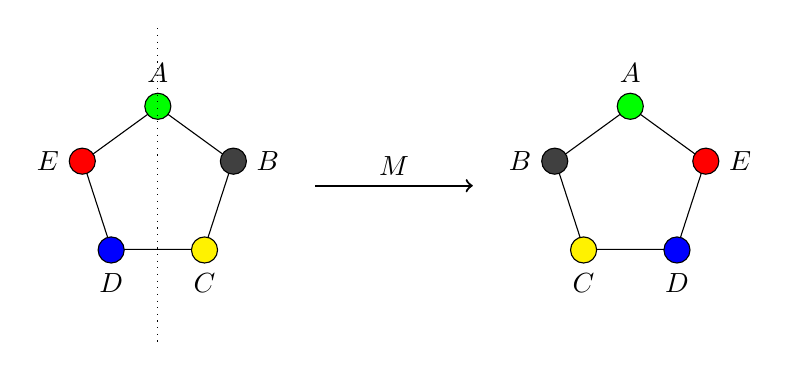
\begin{tikzpicture}
\node[minimum size=2cm,draw,regular polygon,regular polygon sides=5]  at (0,-6) (a) {};
\node[circle,fill=green,radius=.1cm,draw,
    label=above:{$A$}] at (a.corner 1) {};
\node[circle,fill=red, radius=.1cm,draw,
    label=left:{$E$}] at (a.corner 2) {};
\node[circle, fill=blue, radius=.1cm,draw,
    label=below:{$D$}] at (a.corner 3) {};
\node[circle,fill=yellow,radius=.1cm,draw,
    label=below:{$C$}] at (a.corner 4) {};
\node[circle,fill=darkgray,radius=.1cm,draw,
    label=right:{$B$}] at (a.corner 5) {};

    \node[minimum size=2cm,draw,regular polygon,regular polygon sides=5] at (6,-6) (b) {};
\node[circle,fill=green,radius=.1cm,draw,
    label=above:{$A$}] at (b.corner 1) {};
\node[circle,fill=darkgray, radius=.1cm,draw,
    label=left:{$B$}] at (b.corner 2) {};
\node[circle, fill=yellow, radius=.1cm,draw,
    label=below:{$C$}] at (b.corner 3) {};
\node[circle,fill=blue,radius=.1cm,draw,
    label=below:{$D$}] at (b.corner 4) {};
\node[circle,fill=red,radius=.1cm,draw,
    label=right:{$E$}] at (b.corner 5) {};

\draw [thick, ->] (2,-6) -- (4,-6) node[midway, above] {$M$};
\draw[dotted] (0,-4)--(0,-8);
\end{tikzpicture}
\end{frame}

\begin{frame}{Some Observations on $R$ and $M$}
\begin{stepitemize}
\item We first observe that $R^5$ will bring the shape back to its original position, which means $R^5=1$.
\item What happens if we apply the mirror reflection twice?
\item Of course we get the same picture back.
\item In other words $M^2=1$.
\item So the full set of such symmetries will consist of
$1, R, R^2, R^3, R^4, M$ and the possible inter-compositions.
\item So let us look at what happens when we combine $R$ and $M$
\end{stepitemize}
\end{frame}
\begin{frame}{$RM$ vs $MR$}
    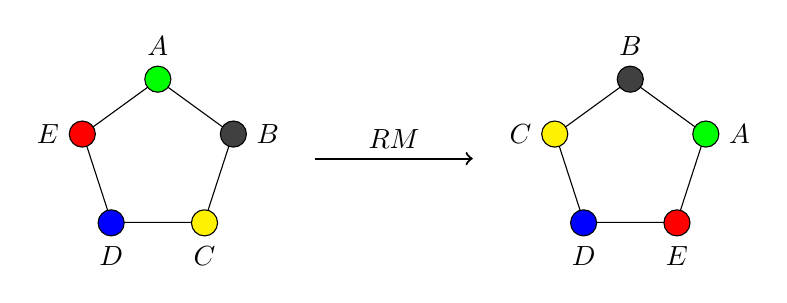
\begin{tikzpicture}
\node[minimum size=2cm,draw,regular polygon,regular polygon sides=5] at (0,0) (a) {};
\node[circle,fill=green,radius=.1cm,draw,
    label=above:{$A$}] at (a.corner 1) {};
\node[circle,fill=red, radius=.1cm,draw,
    label=left:{$E$}] at (a.corner 2) {};
\node[circle, fill=blue, radius=.1cm,draw,
    label=below:{$D$}] at (a.corner 3) {};
\node[circle,fill=yellow,radius=.1cm,draw,
    label=below:{$C$}] at (a.corner 4) {};
\node[circle,fill=darkgray,radius=.1cm,draw,
    label=right:{$B$}] at (a.corner 5) {};


\node[minimum size=2cm,draw,regular polygon,regular polygon sides=5] at (6,0) (b) {};
\node[circle,fill=darkgray,radius=.1cm,draw,
    label=above:{$B$}] at (b.corner 1) {};
\node[circle,fill=yellow, radius=.1cm,draw,
    label=left:{$C$}] at (b.corner 2) {};
\node[circle, fill=blue, radius=.1cm,draw,
    label=below:{$D$}] at (b.corner 3) {};
\node[circle,fill=red,radius=.1cm,draw,
    label=below:{$E$}] at (b.corner 4) {};
\node[circle,fill=green,radius=.1cm,draw,
    label=right:{$A$}] at (b.corner 5) {};

\draw [thick, ->] (2,0) -- (4,0) node[midway, above] {$RM$};
\end{tikzpicture}

\bigskip

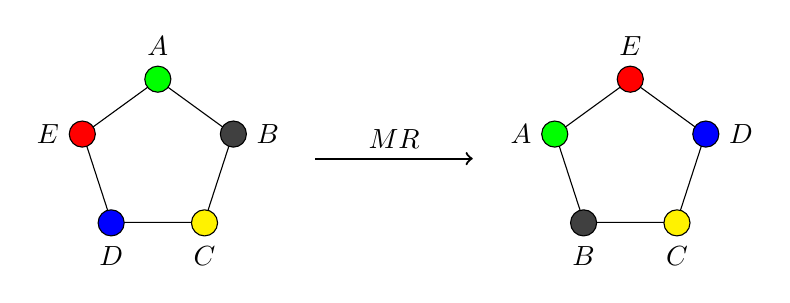
\begin{tikzpicture}
\node[minimum size=2cm,draw,regular polygon,regular polygon sides=5]  at (0,-6) (a) {};
\node[circle,fill=green,radius=.1cm,draw,
    label=above:{$A$}] at (a.corner 1) {};
\node[circle,fill=red, radius=.1cm,draw,
    label=left:{$E$}] at (a.corner 2) {};
\node[circle, fill=blue, radius=.1cm,draw,
    label=below:{$D$}] at (a.corner 3) {};
\node[circle,fill=yellow,radius=.1cm,draw,
    label=below:{$C$}] at (a.corner 4) {};
\node[circle,fill=darkgray,radius=.1cm,draw,
    label=right:{$B$}] at (a.corner 5) {};

    \node[minimum size=2cm,draw,regular polygon,regular polygon sides=5] at (6,-6) (b) {};
\node[circle,fill=red,radius=.1cm,draw,
    label=above:{$E$}] at (b.corner 1) {};
\node[circle,fill=green, radius=.1cm,draw,
    label=left:{$A$}] at (b.corner 2) {};
\node[circle, fill=darkgray, radius=.1cm,draw,
    label=below:{$B$}] at (b.corner 3) {};
\node[circle,fill=yellow,radius=.1cm,draw,
    label=below:{$C$}] at (b.corner 4) {};
\node[circle,fill= blue,radius=.1cm,draw,
    label=right:{$D$}] at (b.corner 5) {};

\draw [thick, ->] (2,-6) -- (4,-6) node[midway, above] {$MR$};

\end{tikzpicture}
\end{frame}

\begin{frame}{More on $M$ and $R$}
\begin{stepitemize}
    \item What do we observe first about $MR$ and $RM$?
    \item We observe that $MR\neq RM$.
    \item However, let us take $RM$ for example:
    \item If we rotate it $3$ more times we get $MR$.
    \item Mathematically, what does that mean?
    \item That $R^3(RM) = R^4M=MR$.
    \item Similarly we can get other relations such as
    $$R^3M=MR^2, \:\: R^2M=MR^3\:\: RM = MR^4.$$
    \item So the whole set of symmetries can be described by $10$ elements:
    $$\{1, R, R^2, R^3, R^4, M, MR, MR^2, MR^3, MR^4\}$$ or
    $$\{1, R, R^2, R^3, R^4, M, RM, R^2M, R^3M, R^4M\}.$$
    \item It does not matter which version you choose, you just need to make sure that you add the condition that $R^iM = MR^{5-i}$.
\end{stepitemize}

\end{frame}


\begin{frame}{Operation Table}
\begin{stepitemize}
\item As we did before, we will look at the operation table of $S = \{1, R, R^2, R^3, R^4, M, MR, MR^2, MR^3, MR^4\}$.

\bigskip

\item[]
\scriptsize{
\begin{center}
\begin{table}[H]
\begin{tabular}{ c| c | c |c|c|c|c|c|c|c|c}
$.$  & $1$ & $R$ & $R^2$ & $R^3$ & $R^4$ & $M$ & $MR$ & $MR^2$ & $MR^3$ & $MR^4$ \\
\hline
$1$ & $1$ & $R$ & $R^2$ & $R^3$ & $R^4$ & $M$ & $MR$ & $MR^2$ & $MR^3$ & $MR^4$ \\
\hline
$R$ & $R$ & $R^2$ & $R^3$ & $R^4$ & $1$ & $MR^4$ & $M$ & $MR$ & $MR^2$ & $MR^3$\\
\hline
$R^2$ & $R^2$ & $R^3$ & $R^4$ & $1$ & $R$ & $MR^3$ & $MR^4$ & $M$ & $MR$ & $MR^2$\\
\hline
$R^3$ & $R^3$ & $R^4$ & $1$ & $R$ & $R^2$ & $MR^2$ & $MR^3$ & $MR^4$ & $M$ & $MR$\\
\hline
$R^4$ & $R^4$ & $1$ & $R$ & $R^2$ & $R^3$ & $MR$ & $MR^2$ & $MR^3$ & $MR^4$ & $M$\\
\hline
$M$ & $M$ & $MR$ & $MR^2$ & $MR^3$ & $MR^4$ & $1$ & $R$ & $R^2$ & $R^3$ & $R^4$\\
\hline
$MR$ & $MR$ & $MR^2$ & $MR^3$ & $MR^4$ & $M$ & $R^4$ & $1$ & $R$ & $R^2$ & $R^3$\\
\hline
$MR^2$ & $MR^2$ & $MR^3$ & $MR^4$ & $M$ & $MR$ & $R^3$ & $R^4$ & $1$ & $R$ & $R^2$\\
\hline
$MR^3$ & $MR^3$ & $MR^4$ & $M$ & $MR$ & $MR^2$ & $R^2$ & $R^3$ & $R^4$ & $1$ & $R$\\
\hline
$MR^4$ & $MR^4$ & $M$ & $MR$ & $MR^2$ & $MR^3$ & $R$ & $R^2$ & $R^3$ & $R^4$ & $1$\\

\end{tabular}
\end{table}

\end{center}
}

\end{stepitemize}

\end{frame}


\section{Groups: Formal definition and Examples}
\begin{frame}{Groups}
    \begin{stepitemize}
    \item The two examples we saw are classical examples of algebraic structures known as ``groups"
    \item In both, we had a way to bring together two elements to get a new element
    \item More precisely we had what is known as a ``binary operation"
    \item The elements of the set obeyed certain rules with regards to the operation.
    \item This is what a group ``roughly" is.
    \item A set of objects with a binary operation and a set of rules that the objects obey with respect to this operation.
    \end{stepitemize}
\end{frame}

\begin{frame}{Formal Definition}
\begin{stepitemize}
    \item Let us start with the formal definition of a group:
 \begin{definition}
Let $G$ be a non-empty set equipped with a binary operation $*$ so that
\begin{enumerate}
    \item $G$ is closed under $*$
    \item $(a*b)*c=a*(b*c)$ for all $a,b,c \in G$
    \item There exists $e\in G$ such that $a*e=e*a=a$ for all $a \in G$ (Identity)
    \item For any $a\in G$, there exists $x\in G$ such that $a*x=x*a=e$ (Inverse Property).
    \item []The pair $(G, *)$ is called a group.
\end{enumerate}
\end{definition}
\item The examples of ``cyclic shifts" and ``symmetries of the pentagon" are both examples of groups.
\item But while in the former case any two elements ``commute", in the latter case we saw that $MR\neq RM$.
\end{stepitemize}
\end{frame}
\begin{frame}{More on groups}
\begin{stepitemize}
\item []{\bf Remark:}
\begin{itemize}
    \item We do not require $a*b=b*a$, however if in a group $G$, $a*b=b*a$ for all $a,b\in G$, then we will call $G$ an ``Abelian group".
    \item We will drop $*$ in most cases. Usually we will either denote the group operation by $.$ or by $+$ depending on the context.
    \item In most examples that we look at, the identity $e$ will be denoted by $1$ or $0$.
    \item The inverse of an element in a group is unique and hence we will denote it by $a^{-1}$ (in an additive group we will denote it by $-a$).
\end{itemize}
\end{stepitemize}

\end{frame}

\begin{frame}{Examples of Groups}
\begin{stepitemize}
\item Here are some examples of groups:
\item $\Z$(Integers), $\Q$(rationals), $\R$ (real numbers), $\C$ (Complex numbers) are all Abelian groups under addition.
    \item $\Z$ is not a group under multiplication as many elements do not have inverses. ($2$ for example).
    \item $\Q$ is not a group under multiplication since $0$ does not have any inverse.
    \item $\Q^{\times} = \Q-\{0\}$ is a group under multiplication. Similarly $\R^{\times}$ and $\C^{\times}$ are also groups under multiplication
    \item For a positive integer $n>1$, we let $\Z_n = \{0,1, \dots, n-1\}$ be the set of residue classes modulo $n$. $\Z_n$ is a group under addition modulo $n$.
    \item For a positive integer $n>1$, we let $\Z_n^{\times} = \{1\leq a \leq n-1|GCD(a,n)=1\}$ be the set of reduced residue classes modulo $n$. $\Z_n^{\times}$ is a group under multiplication modulo $n$.

\end{stepitemize}
\end{frame}
\begin{frame}{More Examples}
  \begin{stepitemize}
    \item The set of $m\times n$ matrices over $\Z$ is an Abelian group under matrix addition.
    \item The set of polynomials with integer coefficients is a group under polynomial addition.
    \item $GL(n;\R) = \{A\in \R^{n\times n}|Det(A) \neq 0\}$, in other words, the set of invertible square matrices over $\R$ is a group under matrix multiplication.
    \item The set of all permutations of $\{1,2, \dots, n\}$ is a group under composition of permutations. We denote this group by $S_n$.

\end{stepitemize}
\end{frame}
\section{Subgroups}
\begin{frame}{Subgroups}
    \begin{stepitemize}
    \item A subgroup is a subset of a group that is a group by itself.
    \item The following theorem explains the main criterion for testing for subgroups:
    \begin{theorem}$($ Subgroup Criterion$)$
Let $G$ be a group and $H$ be a nonempty subset of $G$. $H$ is a subgroup of $G$ (notation: $H\leq G$) if and only if
$$ab^{-1} \in H, \:\: \forall a,b\in H. $$
\end{theorem}

\end{stepitemize}
\end{frame}

\begin{frame}
\begin{stepitemize}
\item Here are some examples:

    \item $2\Z$, or the set of even integers is a subgroup of $\Z$.
    \item $\{1,-1\}$ is a subgroup of $\R^{\times}$ under multiplication
    \item $\{1,-1, i, -i\}$ is a subgroup of $\C^{\times}$ under multiplication
    \item The set of all $n\times n$ matrices whose determinants is $1$ is a subgroup of $GL(n;R)$ that we saw above.
    \end{stepitemize}
\end{frame}

\begin{frame}{Example of a subgroup on the operation table}
\begin{stepitemize}
\item Consider the group $\Z_6$ under addition modulo $6$.
\item Consider the following addition table where we will mark a possible subgroup.
\item[]
\begin{table}[H]
\begin{tabular}{ c| c | c |c|c|c|c}
$\oplus$  & {\color{blue} $0$} & $1$ & {\color{blue} $2$} & $3$ & {\color{blue} $4$} & $5$\\
\hline
{\color{blue} $0$}&{\color{blue} $0$} & $1$ & {\color{blue} $2$} & $3$ & {\color{blue} $4$} & $5$\\
\hline
$1$&$1$ & $2$ & $3$ & $4$ & $5$ & $0$\\
\hline
{\color{blue} $2$} &{\color{blue} $2$} & $3$ & {\color{blue} $4$} & $5$ & {\color{blue} $0$} & $1$\\
\hline
$3$&$3$ & $4$ & $5$ & $0$ & $1$ & $2$\\
\hline
{\color{blue} $4$}&{\color{blue} $4$} & $5$ & {\color{blue} $0$} & $1$ & {\color{blue} $2$} & $3$\\
\hline
$5$&$5$ & $0$ & $1$ & $2$ & $3$ & $4$\\
\end{tabular}
\end{table}
\item Extracting the blue numbers, we get the following table
\item[]
\begin{table}[H]
\begin{tabular}{ c| c | c |c}
$\oplus$  & {\color{blue} $0$} & {\color{blue} $2$} &  {\color{blue} $4$}\\
\hline
{\color{blue} $0$}&{\color{blue} $0$} & {\color{blue} $2$} & {\color{blue} $4$}\\
\hline
{\color{blue} $2$} &{\color{blue} $2$} & {\color{blue} $4$} & {\color{blue} $0$}\\
\hline
{\color{blue} $4$}&{\color{blue} $4$} & {\color{blue} $0$} & {\color{blue} $2$}\\
\end{tabular}
\end{table}
\item So this gives rise to the subgroup $\{0,2,4\}$ of $\Z_6, \oplus)$.
\end{stepitemize}

\end{frame}

\begin{frame}{Another example}
\begin{stepitemize}
\item On the same table we will mark some other numbers
\item[]
\begin{table}[H]
\begin{tabular}{ c| c | c |c|c|c|c}
$\oplus$  & {\color{magenta} $0$} & $1$ & $2$ & {\color{magenta} $3$} &  $4$ & $5$\\
\hline
{\color{magenta} $0$}&{\color{magenta} $0$} & $1$ & $2$ & {\color{magenta} $3$} & $4$ & $5$\\
\hline
$1$&$1$ & $2$ & $3$ & $4$ & $5$ & $0$\\
\hline
 $2$ & $2$ & $3$ & $4$ & $5$ &  $0$ & $1$\\
\hline
{\color{magenta} $3$}& {\color{magenta} $3$} & $4$ & $5$ & {\color{magenta} $0$} & $1$ & $2$\\
\hline
$4$& $4$ & $5$ &  $0$ & $1$ &  $2$ & $3$\\
\hline
$5$&$5$ & $0$ & $1$ & $2$ & $3$ & $4$\\
\end{tabular}
\end{table}
\item Extracting the magenta numbers, we get the following table
\item[]
\begin{table}[H]
\begin{tabular}{ c| c | c}
$\oplus$  & {\color{magenta} $0$} & {\color{magenta} $3$} \\
\hline
{\color{magenta} $0$}&{\color{magenta} $0$} & {\color{magenta} $3$}\\
\hline
{\color{magenta} $3$} &{\color{magenta} $3$} & {\color{magenta} $0$}
\end{tabular}
\end{table}
\item So this gives rise to the subgroup $\{0,3\}$ of $(\Z_6, \oplus)$.
\end{stepitemize}

\end{frame}

\section{Group Homomorphisms}
\begin{frame}{Group Homomorphisms}
\begin{stepitemize}
    \item A homomorphism is a special type of a function that preserves the algebraic structure.
    \item This concept appears in many different algebraic structures.
    \item We will see the group case here.
    \begin{definition}
    Let $(G,.)$ and $(G',*)$ be two groups. A function $\varphi:G\rightarrow G'$ is called a (group) homomorphism if
$$\varphi(g_1g_2) = \varphi(g_1)*\varphi(g_2), \:\:\:\: \forall g_1, g_2 \in G.$$
    \end{definition}
\item In general, if there is no danger of confusion, we will simply denote this concept by
$\varphi(g_1g_2) = \varphi(g_1)\varphi(g_2)$.
\end{stepitemize}

\end{frame}
\begin{frame}{Two Special Sets}
\begin{stepitemize}
    \item There are two special sets related to homomorphisms.
\begin{definition}
Let $\varphi:G\rightarrow G'$ be a group homomorphism.
The ``kernel" of $\varphi$ is defined as
$$ker(\varphi) = \{g\in G|\varphi(g)=e'\},$$
where $e'$ is the identity of $G'$.
Similarly the ``range" is defined as
$$ran(\varphi) = \{\varphi(g)|g\in G\}.$$
\end{definition}

\item Here is an example. Consider $\varphi:\Z_6\rightarrow \Z_6$ given by $\varphi(x)=2x$.

\bigskip
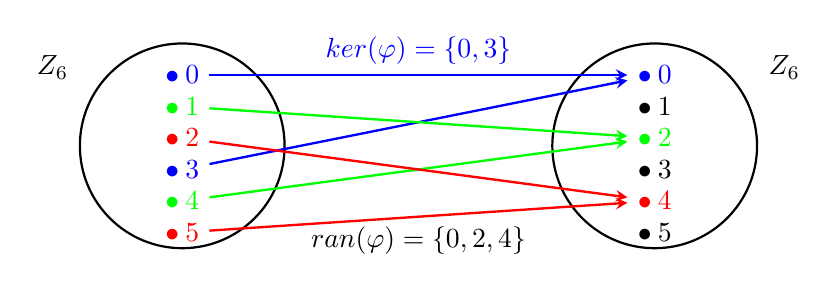
\begin{tikzpicture}[thick,
    set/.style = {circle,
        minimum size = 2cm}]

% Set A
\node[set,label={135:$\Z_6$}] (A) at (-0.6,0) {};

% Set B
\node[set,label={45:$\Z_6$}] (B) at (6.6,0) {};

 \node[text=blue] (v1) at ( 0,0.9)    {$\bullet \:0$};
 \node[text=green] (v2) at ( 0,0.5)    {$\bullet \:1$};
 \node[text=red] (v3) at ( 0,0.1)    {$\bullet \:2$};
 \node[text=blue] (v4) at ( 0,-0.3)    {$\bullet \:3$};
 \node[text=green] (v5) at ( 0,-0.7)    {$\bullet \:4$};
 \node[text=red] (v6) at ( 0,-1.1)    {$\bullet \:5$};
% Intersection
% Circles outline
\draw (0,0) circle(1.3cm);
\draw (6,0) circle(1.3cm);

\node[text=blue] (w1) at ( 6,0.9)    {$\bullet \:0$};
 \node (w2) at ( 6,0.5)    {$\bullet \:1$};
 \node[text=green] (w3) at ( 6,0.1)    {$\bullet \:2$};
 \node (w4) at ( 6,-0.3)    {$\bullet \:3$};
 \node[text=red] (w5) at ( 6,-0.7)    {$\bullet \:4$};
 \node (w6) at ( 6,-1.1)    {$\bullet \:5$};
\draw [-stealth, blue, line width=0.3mm](v1)->(w1) node[midway, above] {$ker(\varphi)=\{0,3\}$};
\draw [-stealth, blue, line width=0.3mm](v4)->(w1);
\draw [-stealth, green, line width=0.3mm](v2)->(w3);
\draw [-stealth, green, line width=0.3mm](v5)->(w3);
\draw [-stealth, red, line width=0.3mm](v3)->(w5);
\draw [-stealth, red, line width=0.3mm](v6)->(w5) node[midway, below, text=black] {$ran(\varphi)=\{0,2,4\}$};
\end{tikzpicture}
\end{stepitemize}

\end{frame}

\begin{frame}{Examples}
\begin{stepitemize}
    \item Let us see some examples:
    \item $\varphi: \Z\rightarrow \Z$ given by $\varphi(m)=2m$
 is a group homomorphism.
Notice that $ker(\varphi) = \{0\}$, while $ran(\varphi) = 2\Z$, i.e., the set of even integers.

 \item In general we can say $\varphi(m)=km$, where $k$ is any integer is also a homomorphism.
 \item $\varphi:\R^{\times} \rightarrow \R^{\times}$ given by $\varphi(x)=\frac{1}{x}$ or $\varphi(x)=x^3$ are examples of homomorphisms (Note that in this case the operation is multiplication). In both cases, the kernel is $\{1\}$, while the range is the full group, i.e., $\R^{\times}$
 \item $\varphi:(\Z,+) \rightarrow (\Z_n, \oplus)$ given by
 $\varphi(m) = (m)_n$, i.e., reduction modulo $n$ is a group homomorphism
 \item $ker(\varphi) = \{m\in \Z| m\equiv 0\pmod{n}\} = n\Z,$
 while $ran(\varphi) = \Z_n$.
\end{stepitemize}

\end{frame}

\begin{frame}{Examples Cont'd}
\begin{stepitemize}
    \item If $G$ is an Abelian group, then $\varphi:G\rightarrow G$ given by $\varphi(g)=g^n$ is a homomorphism.
    \item That us because, if $gh=hg$, then $(gh)^n=g^nh^n$.
    \item However if $G$ is not Abelian, then $\varphi(g)=g^n$ might not be a homomorphism.
    \item To see an example, consider $GL(2;\R)$, namely the group of $2\times 2$ real matrices that are invertible. \item Let $\varphi(g)=g^2$.
 \item Consider
 $$ A=\begin{bmatrix}
    1&0\\
    2&3    \end{bmatrix}, \:\:\: B = \begin{bmatrix}
    -1&2\\
    0&1    \end{bmatrix}.$$
    Then, we have
    \scriptsize{
    $$A^2 = \begin{bmatrix}
    1&0\\
    8&9    \end{bmatrix}, \:\:\: B^2 = \begin{bmatrix}
    1&0\\
    0&1    \end{bmatrix}, \:\:\: AB = \begin{bmatrix}
    -1&2\\
    -2&5    \end{bmatrix}, \:\: A^2B^2 = \begin{bmatrix}
    1&0\\
    8&9    \end{bmatrix}, \:\:\: (AB)^2 = \begin{bmatrix}
    -3&8\\
    -8&21    \end{bmatrix}.$$ }
    \item As we can see $$\varphi(AB) = (AB)^2 \neq A^2B^2 =\varphi(A)\varphi(B).$$
\end{stepitemize}

\end{frame}
\begin{frame}{Examples Cont'd}
\begin{stepitemize}
    \item Here is an interesting example, where the operations could be very different.
    \item Consider the map
$$\varphi: \left( \R, +\right) \rightarrow  \left (\R_{>0}, \cdot \right )$$ given by
$\varphi(x)=2^x$.
\item Since $2^{x+y} = 2^x\cdot 2^y$, this is a homomorphism. \item Moreover, $ker(\varphi) = \{0\}$ while $ran(\varphi) = \R_{>0}$

\end{stepitemize}
\end{frame}

\begin{frame}{Examples Cont'd}
    \begin{stepitemize}
\item Recall that the RSA encryption is a modular exponentiation in $\Z_n^{*}$.
\item An element $m\in \Z_n^*$ is encrypted by $m^e
\pmod{n}$.
\item This operation is homomorphic since $(m_1m_2)^e \equiv m_1^em_2^e \pmod{n}$.
\item This shows that the RSA encryption is a ``partially homomorphic" encryption.

\end{stepitemize}

\end{frame}

\section{Isomorphisms}
\begin{frame}{Isomorphisms}
\begin{stepitemize}
\item  A homomorphism $\varphi:G\rightarrow G'$ is called an ``isomorphism" if it is one-to-one and onto.
\item If there is an isomorphism between $G$ and $G'$ we call the groups ``isomorphic" and we denote it by $G\simeq G'$.
\item  Isomorphic groups essentially have an identical structure and they are considered indistinguishable in Algebra.
 \item $(\Z, +) \simeq (2\Z, +)$ as the homomorphism $\varphi(m)=2m$ is in fact an isomorphism.
     \item $(\R, +) \simeq (\R_{>0},\cdot)$ since the homomorphism $\varphi(x) = 2^x$ is indeed an isomorphism.
\end{stepitemize}
\end{frame}

\section{Cosets, Lagrange's Theorem}
\begin{frame}{Cosets}
    \begin{stepitemize}
    \item If $H$ is a subgroup $aH = \{ah|h\in H\}$
is called a left coset of $H$ in $G$.
\item Cosets are equivalence classes under the equivalence relation $a\sim b$ if and only if $a^{-1}b \in H$.
    \item As equivalence classes, they partition the whole group into cosets. In other words, the group $G$ is a union of these left cosets and any two left cosets are either identical or disjoint.


\bigskip
\item[]
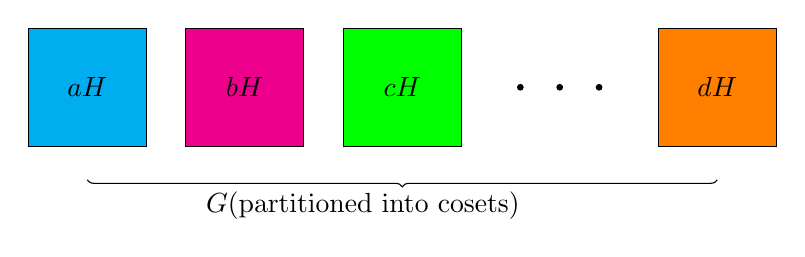
\begin{tikzpicture}
    \node[rectangle, draw,  fill=cyan, minimum width = 1.5cm,
    minimum height = 1.5 cm](r1) at (-2,0){$aH$};
    \node[rectangle, draw,  fill=magenta, minimum width = 1.5cm,
    minimum height = 1.5 cm](r2) at (0,0){$bH$};
    \node[rectangle, draw, fill=green, minimum width = 1.5cm,
    minimum height = 1.5 cm](r3) at (2,0){$cH$};
    \tikzstyle{point2}=[ball color=green, circle, draw=black, inner sep=0.1cm]
    \filldraw[black] (3.5,0) circle (1pt);

\filldraw[black] (4,0) circle (1pt);

\filldraw[black] (4.5,0) circle (1pt);

\node[rectangle, draw,  fill = orange, minimum width = 1.5cm,
    minimum height = 1.5 cm](r4) at (6,0){$dH$};

    \draw[decoration={brace,mirror,raise=5pt},decorate]
  (-2,-1) -- node[below=3pt] {} (6,-1);

\node[] at (1.5,-1.5){$G$(partitioned into cosets)};
\end{tikzpicture}

\end{stepitemize}

\end{frame}

\begin{frame}{Lagrange}
\begin{stepitemize}
    \item For two cosets $aH$ and $bH$, the map
    $f:aH\rightarrow bH, \:\:\: f(x) = b(a^{-1}x)$
is a bijection (one-to-one correspondence).

    \item An important consequence of this is that when $G$ is finite, any two cosets have the same size.
    \item Since $G$ is a disjoint union of the cosets, we get the following theorem:
\begin{theorem}$($Lagrange's Theorem $)$
If $G$ is a finite group, and $H$ is any subgroup then we must have $|H| \: | \: |G|$.
\end{theorem}
\item This gives us the set of all possible sizes for subgroups of a group.
\item So that for example we know a group of size $10$ cannot have a subgroup of size $3$ or $4$.
\end{stepitemize}

\end{frame}

\begin{frame}{Examples of Cosets}
    \begin{stepitemize}
        \item Let $\Z$ be the group and we take the subgroup to be $3\Z$.
        \item Then the set of all cosests is given by
    $3\Z, 1+3\Z, 2+3\Z$.
    \item Note that $3+3\Z$ is the same as $3\Z$ and $4+3\Z$ is the same as $1+3\Z$, etc.
    \item They partition the group of all integers as any integer must belong to one of these cosets. (Recall, the remainder upon dividing an integer by 3 is 0, 1 or 2. )
    \item The following is a picture of this partitioning:

    \bigskip

    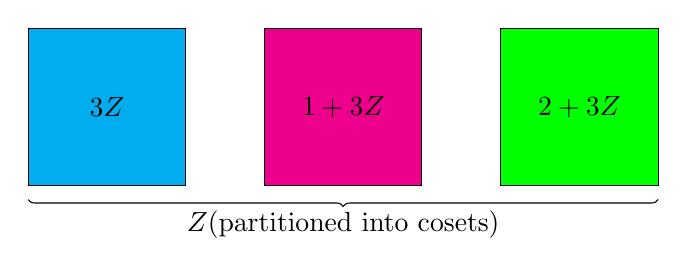
\begin{tikzpicture}
    \node[rectangle, draw,  fill=cyan, minimum width = 2cm,
    minimum height = 2 cm](r1) at (0,0){$3\Z$};
    \node[rectangle, draw,  fill=magenta, minimum width = 2cm,
    minimum height = 2 cm](r2) at (3,0){$1+3\Z$};
    \node[rectangle, draw, fill=green, minimum width = 2cm,
    minimum height = 2 cm](r3) at (6,0){$2+3\Z$};

    \draw[decoration={brace,mirror,raise=5pt},decorate]
  (-1,-1) -- node[below=3pt] {} (7,-1);

\node at (3,-1.5){$\Z$(partitioned into cosets)};
\end{tikzpicture}

    \end{stepitemize}
\end{frame}

\begin{frame}{Another Example}
\begin{stepitemize}
    \item Let $G=\Z_{8}^{\times} = \{1,3,5,7\}$ and let $H = \{1,3\}$.
    \item Then there will be $2$ distinct cosets of $H$ in $G$ and they will be given by $H = \{1,3\}$ and $5H = \{5, 15\} \equiv \{5,7\} \pmod{8}$.
    \item Note that $3H = H$ and $7H=5H$.
    \item[]

    \bigskip

    \begin{tikzpicture}
    \node at (0,2){$H$};
    \node at (6,2){$5H$};
    \node at (0,1){$\bullet \:1$};
    \node at (0,-1){$\bullet \:3$};
    \node at (6,1){$\bullet \:5$};
    \node at (6,-1){$\bullet \:7$};
    \node[rectangle, draw,  minimum width = 3cm,
    minimum height = 3 cm](r1) at (0,0){};
    \node[rectangle, draw, minimum width = 3cm,
    minimum height = 3 cm](r2) at (6,0){};

\draw[decoration={brace,mirror,raise=5pt},decorate]
  (-1,-2) -- node[below=3pt] {} (7,-2);

\node at (3,-3){$\Z_8^*$(partitioned into cosets)};
\end{tikzpicture}
\end{stepitemize}
\end{frame}

\section{Order of Elements, Cyclic groups and Discrete Logarithm Problem}
\begin{frame}{Order of an Element}
    \begin{stepitemize}
    \item Similar to what we saw in Number Theory
    \item In general we have the following definition:
    \begin{definition}
Let $G$ be a group and $g\in G$ be any element. The order $g$, denoted $ord(g)$ is the smallest positive integer $n$ such that $g^n=e$. In other words, $ord(g)=n$ if
\begin{enumerate}
    \item $g^n=e$, and
    \item $g^h\neq e$, if $1\leq h <n$.
\end{enumerate}
\end{definition}

\item[] \begin{lemma}\label{1}
If $ord(g) = n$, then $e, g, g^2, \dots, g^{n-1}$ are all distinct.
\end{lemma}

\item[] \begin{corollary}
Since $\{e,g, \dots, g^{n-1}\} \subseteq G$, this means that $ord(g)\leq |G|.$
\end{corollary}
\end{stepitemize}
\end{frame}
\begin{frame}{More on Order}
\begin{stepitemize}
    \item[] \begin{lemma}
If $ord(g)=n$, then $g^m=e$ if and only if $n|m$.
\end{lemma}
\item In fact we have the following theorem on order:
\begin{theorem}
If $G$ is a finite group and $g \in G$ is any element, then
$ord(g)| \: |G|$.
\end{theorem}
\item Here are some examples:
\begin{enumerate}
    \item In any group $G$, $ord(g)=1$ if and only if $g=e$.
    \item In $(\Z_6,\oplus)$, $ord (0)=1$, $ord(1)=ord(5)=6$, $ord(2)=ord(4)=3$ and $ord(3)=2$.
    \item In $\Z_{8}^{\times}$, $ord(1)=1$, $ord(3)=ord(5)=ord(7)=2$ since $3^2\equiv 5^2\equiv 7^2 \equiv 1 \pmod{8}$.
\end{enumerate}
\end{stepitemize}

\end{frame}

\begin{frame}{Cyclic Groups}
    \begin{stepitemize}
    \item Cyclic groups are special as they are generated by a single element
    \item A group $G$ is cyclic if there exists $g\in G$ such that
$$G = \langle g\rangle = \{g^n|n\in \Z\}.$$
\item $(\Z,+)$ is cyclic and is generated by $1$.
    \item $(\Z_n, \oplus)$ is also cyclic and is generated by $1$.
    \item $\Z_7^{\times} = \{1,2,3,4,5,6\}$ is cyclic and is generated by $3$ since
    $$\langle3\rangle = \{1,3,3^2, 3^3, 3^4, 3^5\} \equiv \{1,3,2,6,4,5\} \pmod{7}.$$
    \item $\Z_8^{\times} = \{1,3,5,7\}$ is not a cyclic group since $3^2\equiv 5^2\equiv 7^2\equiv 1 \pmod{8}$.
    \end{stepitemize}
\end{frame}

\begin{frame}{The Discrete Logarithm Problem}
    \begin{stepitemize}
    \item Cyclic groups play a crucial role in many cryptographic applications.
    \item One of the prominent such examples is the discrete logarithm problem which was the basis of public key cryptography.
    \item The main set up of the problem can be described as follows:

\item Let $G$ be a cyclic group generated by some $g$ (Usually $G$ is taken to be $\Z_p^{\times}$, where $p$ is a large prime).
\item The discrete logarithm of an element $h\in G$ is $m\in \Z_+$ such that $g^m=h$.
\item The discrete logarithm problem is the problem of determining $m$ from the knowledge of $g$ and $h$.

    \end{stepitemize}
\end{frame}

\begin{frame}{Diffie-Helman Key Exchange}
\begin{stepitemize}
\item Alice and Bob have access to the generator $g$ of a cyclic group $G$.
\item They each have their private keys, which will be denoted by $a$ and $b$, respectively.
\item The idea is to secure a common key for Alice and Bob that they can use as a session key.
\item So, Alice sends $g^a$ to Bob, while Bob sends $g^b$ to Alice.
\item Alice then uses her key on $g^b$, namely she calculates
$(g^b)^a$, while Bob uses his key on $g^a$, namely he calculates $(g^a)^b$.
\item Of course we have
$$(g^b)^a=g^{ba} = g^{ab}=(g^a)^b.$$

\item Thus Alice and Bob have secured a common key without danger from the eavesdropper thanks to the difficulty of the Discrete Logarithm Problem.
\end{stepitemize}
\end{frame}

\begin{frame}{A Toy Example}
\begin{stepitemize}
\item Consider the cyclic group
$\Z_{10529}^{\times} = \{1, 2, \dots, 10528\}. $
\item It turns out that $17$ is a primitive element modulo $10529$, so the group is generated by $17$.
 \item Alice chooses $656$ as her secret key and Bob chooses $1879$ as his secret key.
 \item The following describes how they achieve a common session key:
 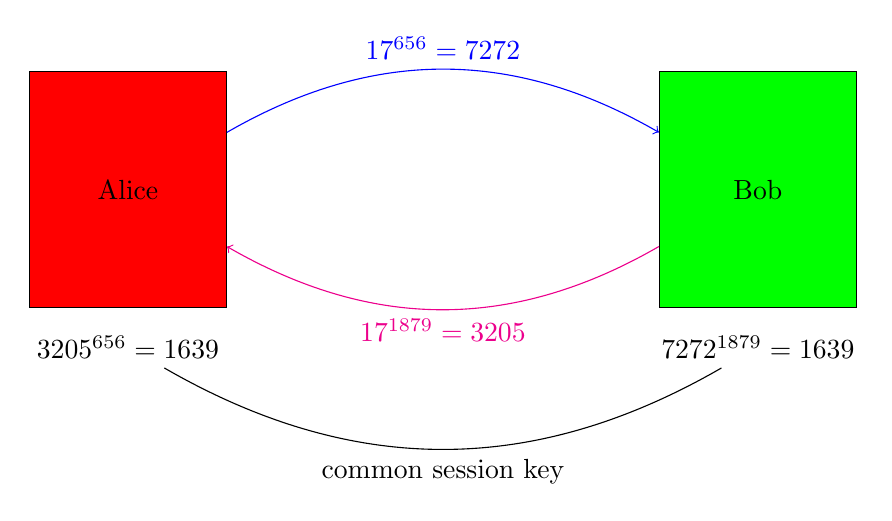
\begin{tikzpicture}
\node[fill=red, text=black, rectangle,draw,  minimum width = 2.5cm,
    minimum height = 3cm] (r1) at (0,0) {Alice};

 \node[fill=green, text=black,rectangle,draw,  minimum width = 2.5cm,
    minimum height = 3cm] (r2) at (8,0) {Bob};
\draw[->,bend left, blue] (r1) edge node[above]{$17^{656} = 7272$}(r2);
\draw[->,bend left, magenta]  (r2) edge node[below]{$17^{1879} = 3205$}(r1);

\node (s1)at (0,-2){$3205^{656} = 1639$};
\node (s2)at (8,-2){$7272^{1879} = 1639$};

\draw[bend right]  (s1) edge node[below]{common session key}(s2);

\end{tikzpicture}

\end{stepitemize}

\end{frame}

\section{Factor Groups and Isomorphism Theorems}

\begin{frame}{Factor Groups}
    \begin{stepitemize}
    \item Factor groups are a way to generate new groups from existing groups.
    \item We take the cosets to be the elements.
    \item Notation: $G/H = \{gH|g\in G\}$.
    \item To turn $G/H$ into a group we need to define an operation.
    \item The natural choice is to define $(aH)(bH) = (ab)H$.
    \item For this to be well-defined, the subgroup needs to have some special properties.
    \item Formally, the subgroup has to be normal
    \item Since we will mostly consider Abelian groups, we should note that all subgroups of Abelian groups are normal.
    \end{stepitemize}
\end{frame}

\begin{frame}{Example}
\begin{stepitemize}
\item Consider $G = \Z$ and let $H=3Z$.
\item Then $G/H = \{3\Z, 1+3\Z, 2+3\Z\}$.
\item The operations then can be described as
$$(1+3\Z)+(2+3\Z) = 3+3\Z = 3\Z, \:\:\:\: (1+3\Z)+(1+3\Z) = 2+3\Z, \dots$$
\item Notice that the coset $3\Z$ acts as the identity element.
\item It is not hard to see that $G/H$ acts very similar to $(\Z_3, \oplus)$.
\item This is not a coincidence as we will see from the 1st isomorphism theorem.
\end{stepitemize}
\end{frame}
\begin{frame}{Factor Group}
\begin{stepitemize}
\item To better see the similarity, we look at the operation tables of the two groups:
\item[]
\begin{columns}
        \begin{column}{0.4\textwidth}
            \begin{table}
            \begin{tabular}{ c| c | c |c}
$\oplus$  & {\color{darkgray} $3\Z$} & {\color{blue} $1+3\Z$} &  {\color{red} $2+3\Z$}\\
\hline
{\color{darkgray} $3\Z$}&{\color{darkgray} $3\Z$} & {\color{blue} $1+3\Z$} & {\color{red} $2+3\Z$}\\
\hline
{\color{blue} $1+3\Z$} &{\color{blue} $1+3\Z$} & {\color{red} $2+3\Z$} & {\color{darkgray} $3\Z$}\\
\hline
{\color{red} $2+3\Z$}&{\color{red} $2+3\Z$} & {\color{darkgray} $3\Z$} & {\color{blue} $1+3\Z$}
\end{tabular}

            \caption{The group $\Z/3\Z$}
            \end{table}
        \end{column}
        \begin{column}{0.3\textwidth}
            \begin{table}
            \begin{tabular}{ c| c | c |c}
$\oplus$  & {\color{darkgray} $0$} & {\color{blue} $1$} &  {\color{red} $2$}\\
\hline
{\color{darkgray} $0$}&{\color{darkgray} $0$} & {\color{blue} $1$} & {\color{red} $2$}\\
\hline
{\color{blue} $1$} &{\color{blue} $1$} & {\color{red} $2$} & {\color{darkgray} $0$}\\
\hline
{\color{red} $2$}&{\color{red} $2$} & {\color{darkgray} $0$} & {\color{blue} $1$}
\end{tabular}
            \caption{The group $\Z_3$}
            \end{table}
        \end{column}
    \end{columns}

\end{stepitemize}

\end{frame}

\begin{frame}{1st Isomorphism Theorem}
\begin{stepitemize}
\item The first isomorphism theorem formalizes our observation of how $\Z/3\Z$ acts like $\Z_3$:
\begin{theorem}$($1st Isomorphism Theorem $)$
Let $\varphi: G\rightarrow G'$ be a homomorphism. Then we have
$$G/ker(\varphi) \simeq ran(\varphi).$$
\end{theorem}
\item To formalize our previous observation, consider the homomorphism $\varphi:(\Z,+) \rightarrow (\Z_3, \oplus)$ given by $\varphi(m) = (m)_3$.
\item Then $ker(\phi) = 3\Z$, that is all multiples of $3$ while $ran(\phi) = \Z_3$.
\item Thus from the theorem we can say
    $$\Z/3\Z \simeq \Z_3.$$
\end{stepitemize}
\end{frame}

\begin{frame}{Another Example}
\begin{stepitemize}
    \item Let us consider one last example.
    \item Consider $\varphi:\R[x]\rightarrow \R$ given by $\varphi(p(x)) = p(0)$.
    \item We can see that $ker(\varphi) = x\R[x]$, while $ran(\varphi)=\R$.
    \item Thus by the theorem we have
    $$\R[x]/(x\R[x]) \simeq \R.$$
    \item We can interpret this isomorphism as ``killing" the $x$ term when we factor, thus leaving us with only the constant terms.
\end{stepitemize}
\end{frame}
\begin{frame}

\centerline{ \color{blue} \bf{\large THANK YOU!!!}}

\end{frame}

\end{document}
